%------------------------------------------------
% main.tex - test file for camel.cls
%------------------------------------------------
\documentclass{camel}
\usepackage{camel}

\academicyear{2014-15}
\modulecode{MA0000}
\moduletitle{Test Module}
\booktitle{Notes}

\usepackage{caption}
\usepackage{subcaption}
\captionsetup[subfigure]{labelformat=empty}
\captionsetup[figure]{skip=2ex}
\RequirePackage{graphicx}
\graphicspath{{./figures/}}
\DeclareGraphicsExtensions{.pdf,.jpeg,.png,.gif}

\def\it{\item}
\def\bit{\begin{itemize}}
\def\eit{\end{itemize}} 
\def\ben{\begin{enumerate}}
\def\een{\end{enumerate}}

\newcommand{\N}{\mathbb{N}}
\newcommand{\Z}{\mathbb{Z}}
\newcommand{\Q}{\mathbb{Q}}
\newcommand{\R}{\mathbb{R}}
\newcommand{\C}{\mathbb{C}}
\newcommand{\prob}{\mathbb{P}}
\newcommand{\expe}{\mathbb{E}}
\newcommand{\var}{\text{Var}}
\newcommand{\cov}{\text{Cov}}


%----------------------------------------------------------------------
\begin{document}
\makefrontmatter
%----------------------------------------------------------------------

% Anything before the first chapter causes a spurious entry in list of chapters

%----------------------------------------------------------------------
\chapter{Divisions}\label{ch:divisions}
%----------------------------------------------------------------------

Some initial text, before the first section
%---------------------------------------
\section{First Section}
%---------------------------------------
This is the first section.

%---------------------------------------
\section{Another Section}
%---------------------------------------
This is the second section.


% subsection not implemented yet (not difficult)
%---------------------------------------
%\subsection{A subsection}
%---------------------------------------
%This is a subsection.

%----------------------------------------------------------------------
\chapter{Exercises}\label{ch:exercises}
%----------------------------------------------------------------------

\bit
\it Doesn't work across chapters yet: Lemma~\ref{lem:zorn}.
\eit
%---------------------------------------
\section{Diagnostic exercises (multiple choice)}
%---------------------------------------
\begin{diagnostic}\label{dex:demo}
\begin{questions}
\question Which among the following distributions is the odd one out? \label{qu:dex:demo:first-question}
\begin{choices}
\choice Binomial
\correctchoice Exponential
\choice Geometric
\choice Poisson
\end{choices}
\question Which is the definition of a random variable? \label{qu:dex:demo:second-question}
\begin{choices}
\correctchoice A function $X:\Omega\to\R$.
\choice A function $X:\Omega\to[0,1]$.
\choice A function $X:\R\to[0,1]$.
\end{choices}
\end{questions}
\end{diagnostic}

%---------------------------------------
\section{Formative exercises}
%---------------------------------------
\begin{formative}\label{fex:demo}
This is the introduction.
\begin{questions}
\question This is the first question.\label{qu:fex:demo:first-question}
\begin{answer}
This is the answer to the first question.
\end{answer}
\question This is the second question.\label{qu:fex:demo:second-question}
\begin{answer}
This is the answer to the second question.
\end{answer}
\question This is the third question.\label{qu:fex:demo:third-question}
\begin{parts}
\part This is the first part of the third question
\begin{answer}
This is the answer to the first part of the third question.
\end{answer}
\part This is the second part of the third question
\begin{answer}
This is the answer to the second part of the third question.
\end{answer}
\end{parts}
\end{questions}
\end{formative}

%----------------------------------------------------------------------
\chapter{Figures and Tables}\label{ch:figsures_and_tables}
%----------------------------------------------------------------------

%----------------------------------------------------------------------
\section{Figures}\label{sec:figures}
%----------------------------------------------------------------------
Not done yet.

\begin{figure}[htb]
\centering
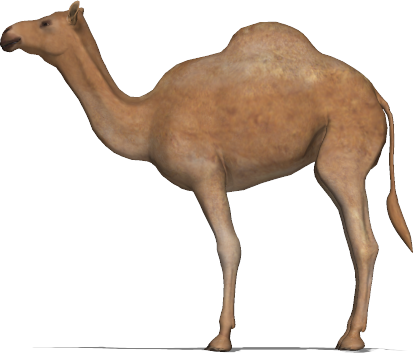
\includegraphics[scale=0.25]{figures/humpty.png}
\caption{Humpty the Camel.}
\label{humpty-the-camel}
\end{figure}

%----------------------------------------------------------------------
\section{Tables}\label{sec:tables}
%----------------------------------------------------------------------
Here are some tables:

\begin{table}
\begin{tabular}{ll}\hline
Notation		& $X\sim\text{Uniform}\{1,2,\ldots,n\}$ \\
Parameter(s)	& $n\in\mathbb{N}$ \\
Range			& $\{1,2,\ldots,n\}$ \\
PMF				& $f(k) = 1/n$ for all $k=1,2,\ldots,n$ \\ \hline
\end{tabular}
\caption{The uniform distribution}
\end{table}

\begin{table}
\begin{tabular}{ll}\hline
Notation			& $X\sim\text{Bernoulli}(p)$ \\
Parameter(s)		& $p \in [0,1]$ \quad (probability of success) \\
Range			& $\{0,1\}$ \\
PMF				& $f(0) = 1-p$ and $f(1) = p$ \\ \hline
\end{tabular}
\caption{The Bernoulli distribution}
\end{table}

%----------------------------------------------------------------------
\chapter{Theorems}\label{ch:theorems}
%----------------------------------------------------------------------
Probability is a \emph{function} that assigns numerical value to random events.

\begin{definition}\label{def:prob_measure}
Let $\Omega$ be the sample space of some random experiment, and let $\mathcal{F}$ be a field of sets over $\Omega$. A \emph{probability measure} on $(\Omega,\mathcal{F})$ is a function
\[
\begin{array}{rccl}
	\prob:	& \mathcal{F}	& \to	& [0,1] \\[1ex]
			& A				& \mapsto	& \prob(A)
\end{array}
\]
such that $\prob(\Omega) = 1$, and for any countable collection of pairwise disjoint events $\{A_1,A_2,\ldots\}$,
\[
\prob\left(\bigcup_{i=1}^\infty A_i\right) = \sum_{i=1}^{\infty} \prob(A_i).
\]
The triple $(\Omega,\mathcal{F},\prob)$ is called a \emph{probability space}.
\end{definition}

% theorem: properties of probability measures
\begin{theorem}[Properties of probability measures]\label{thm:properties_of_probability_measures}
Let $(\Omega,\mathcal{F},\prob)$ be a probability space, and let $A,B\in\mathcal{F}$. 
\ben
\it Complementarity: $\prob(A^c) = 1 - \prob(A)$.
\it $\prob(\emptyset) = 0$,
\it Monotonicity: if $A\subseteq B$ then $\prob(A)\leq \prob(B)$.
\it Addition rule: $\prob(A\cup B) = \prob(A) + \prob(B) - \prob(A\cap B)$.
\een
\end{theorem}
% proof
\begin{proof}
\ben
\it % complementarity
Since $A\cup A^c=\Omega$ is a disjoint union and $\prob(\Omega)=1$, it follows by additivity that 
\[
1 = \prob(\Omega) = \prob(A\cup A^c) = \prob(A) + \prob(A^c).
\]
\it % emptyset
Since $\emptyset=\Omega^c$ and $\prob(\Omega)=1$, it follows by complemenarity that
\[
\prob(\emptyset) = \prob(\Omega^c) = 1 - \prob(\Omega) = 1 - 1 = 0.
\]
\it % monotonicity
Let $A\subseteq B$ and let us write $B = A\cup (B\setminus A)$. 

Since $A$ and $B\setminus A$ are disjoint sets, it follows by additivity that
\[
\prob(B) = \prob\big[A\cup (B\setminus A)\big] = \prob(A) + \prob(B\setminus A).
\]
Hence, because $\prob(B\setminus A)\geq 0$, it follows that $\prob(B) \geq \prob(A)$.

\it % addition rule
\bit
\it $A\cup B = (A\setminus B) \cup (B\setminus A) \cup (A\cap B)$
\it $A 		 = (A\setminus B) + (A\cap B)$
\it $B 		 = (B\setminus A) + (A\cap B)$
\eit
These are disjoint unions, so by additivity, 
\bit
\it $\prob(A\cup B) = \prob(A\setminus B) + \prob(B\setminus A) + \prob(A\cap B)$
\it $\prob(A) 		= \prob(A\setminus B) + \prob(A\cap B)$
\it $\prob(B)		= \prob(B\setminus A) + \prob(A\cap B)$
\eit
Hence $\prob(A\cup B) = \prob(A) + \prob(B) - \prob(A\cap B)$, as required.
\een
\end{proof}

Here is a lemma:
\begin{lemma}[Zorn's lemma]\label{lem:zorn}
If every totally ordered subset of a partially ordered set $A$ has an upper bound in $A$, then $A$ contains at least one maximal element.
\end{lemma}

%----------------------------------------------------------------------
\chapter{Lists}\label{ch:lists}
%----------------------------------------------------------------------
Here are nested itemize environments
\begin{itemize}
\item First item
	\begin{itemize}
	\item First sub-item
	\item Second sub-item
	\end{itemize}
\item Second item
\end{itemize}

Here are nested enumerate environments
\begin{enumerate}
\item First item
	\begin{enumerate}
	\item First sub-item
	\item Second sub-item
	\end{enumerate}
\item Second item
\end{enumerate}

%----------------------------------------------------------------------
\chapter{Labels, References and Citations}
%----------------------------------------------------------------------
\bit
\it Here is a reference to Lemma~\ref{lem:zorn} -- does it work?
\it Here is a reference to Definition~\ref{def:prob_measure} -- does it work?
\eit


%----------------------------------------------------------------------
\chapter{camel.cls documentation}\label{chap:camelcls}
%----------------------------------------------------------------------
\bit
\it Options: 
\it Show/Hide



%----------------------------------------------------------------------
\end{document}
%----------------------------------------------------------------------

